\section{Documentación de la Implementación Estudiante - Profesión}

Se desarrola el proyecto en Java, creando este proyecto mediante el IDE de NetBeans y para la codificación me apoyo sobre el editor de Visual Studio Code, el cual me permite escribir código de manera más fluida y con una mejor experiencia de usuario. Para la documentación del proyecto, se utiliza LaTeX, un sistema de preparación de documentos que es ampliamente utilizado en el ámbito académico y científico debido a su capacidad para manejar fórmulas matemáticas complejas y su alta calidad tipográfica.

\subsection{Creación del Proyecto}

\begin{figure}[H]
  \centering
  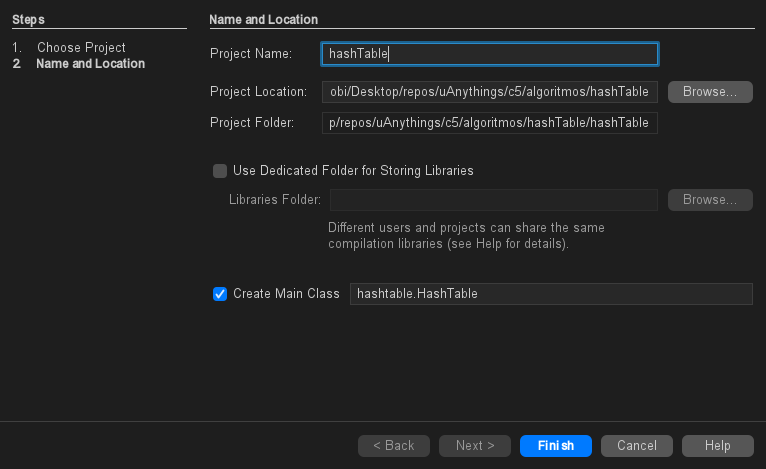
\includegraphics[width=0.6\textwidth]{assets/a1.png}
  \caption{Creación del proyecto en NetBeans}
  \label{fig:project-creation}
\end{figure}

Se realizará ambas implementaciones bajo un mismo proyecto.

\subsection{Creación de la interfaz con JFrame Form}

\begin{figure}[H]
  \centering
  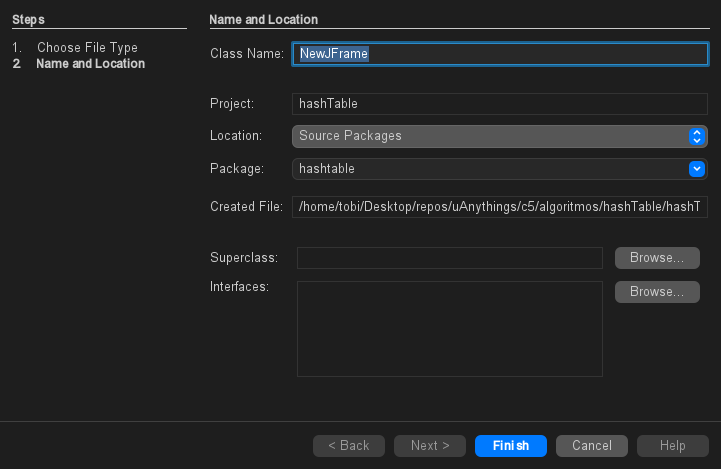
\includegraphics[width=0.6\textwidth]{assets/a2.png}
  \caption{Creación de la interfaz con JFrame Form}
  \label{fig:jframe-creation}
\end{figure}

\subsection{Generación de la interfaz}

\begin{figure}[H]
  \centering
  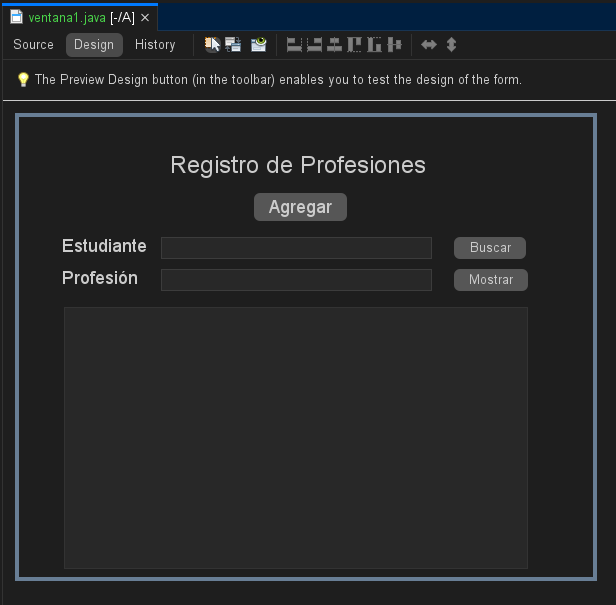
\includegraphics[width=0.5\textwidth]{assets/a3.png}
  \caption{Generación de la interfaz}
  \label{fig:interface-generation}
\end{figure}

Se crea una interfaz gráfica utilizando JFrame Form, lo que permite una interacción más amigable con el usuario y facilita la visualización de los datos almacenados en las tablas hash. Esta se llama Ventana 1.

\subsection{Botón de agregar}

\begin{figure}[H]
  \centering
  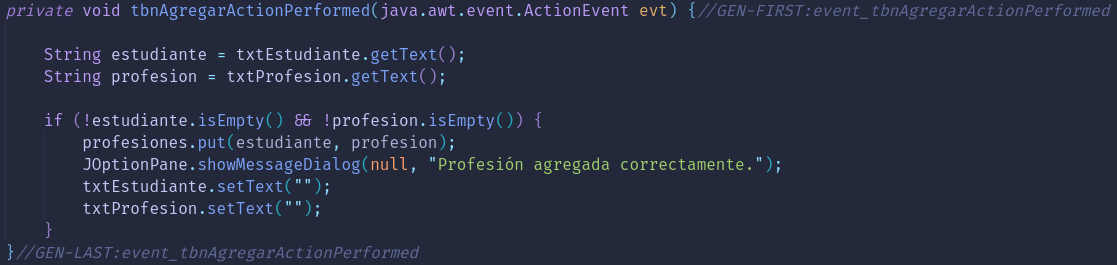
\includegraphics[width=1\textwidth]{assets/a4.png}
  \caption{Botón de agregar}
  \label{fig:add-button}
\end{figure}

\subsection{Botón de buscar}

\begin{figure}[H]
  \centering
  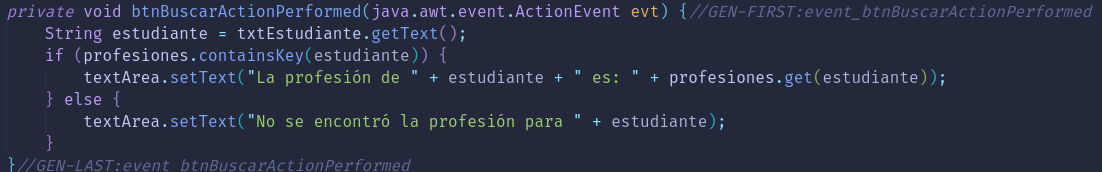
\includegraphics[width=1\textwidth]{assets/a5.png}
  \caption{Botón de buscar}
  \label{fig:search-button}
\end{figure}

\newpage

\subsection{Botón de mostrar}

\begin{figure}[H]
  \centering
  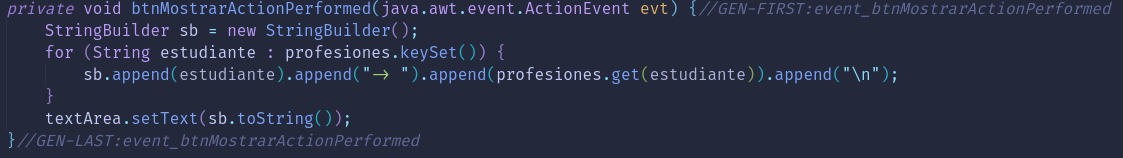
\includegraphics[width=1\textwidth]{assets/a6.png}
  \caption{Botón de mostrar}
  \label{fig:show-button}
\end{figure}

\subsection{Agregar datos}

Se agregan datos a la tabla hash de acuerdo al requerimiento del proyecto, lo solicitado son 20 registros y 3 simulaciones de búsqueda.

\begin{figure}[H]
  \centering
  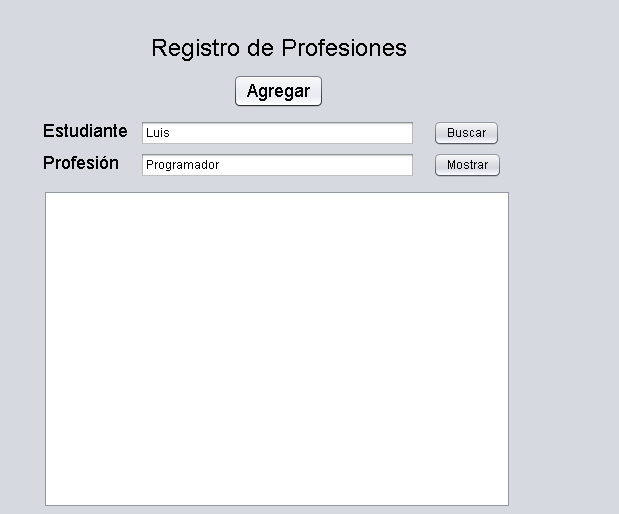
\includegraphics[width=0.8\textwidth]{assets/a7.png}
  \caption{Agregar datos}
  \label{fig:add-data}
\end{figure}
\begin{figure}[H]
  \centering
  
\includegraphics[width=0.4\textwidth]{assets/a8.png}
  \caption{Éxito al agregar datos}
  \label{fig:add-data-muestra}
\end{figure}

\subsection{Muestra de 20 Registros}
\begin{figure}[H]
  \centering
  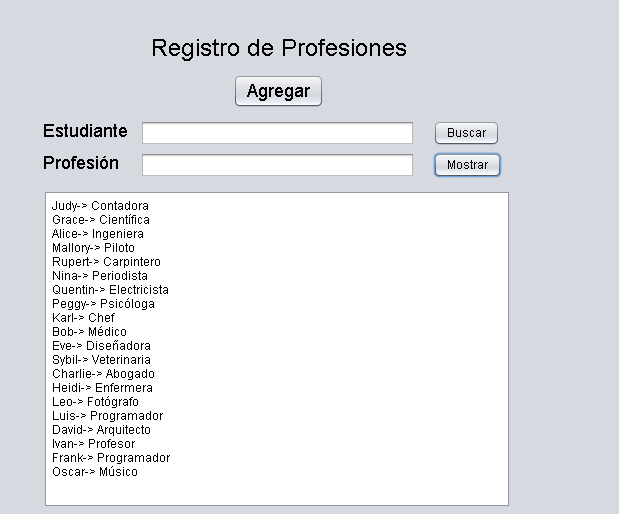
\includegraphics[width=0.7\textwidth]{assets/a9.png}
  \caption{Muestra de 20 registros}
  \label{fig:show-data}
\end{figure}

\subsection{Muestra de 3 búsquedas}
\begin{figure}[H]
  \centering
  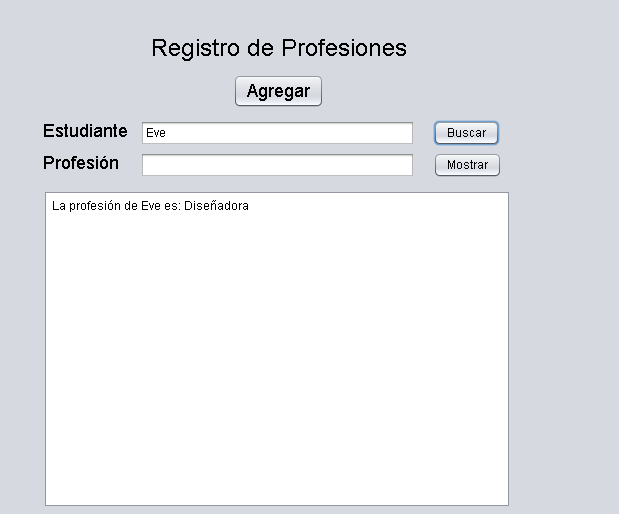
\includegraphics[width=0.7\textwidth]{assets/a10.png}
  \caption{Primera muestra}
  \label{fig:search-data}
\end{figure}
\begin{figure}[H]
  \centering
  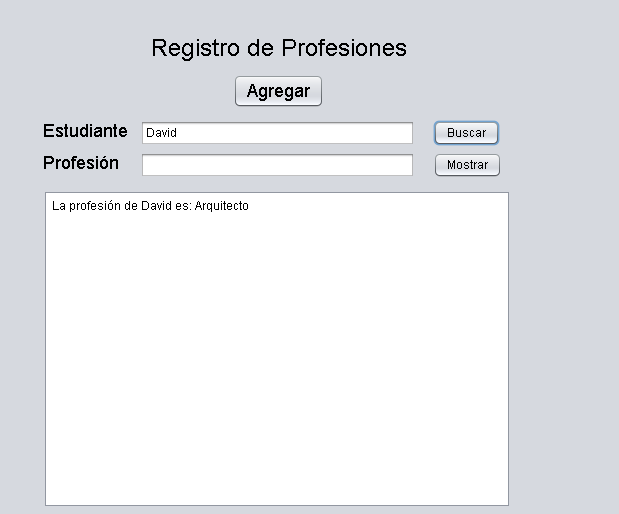
\includegraphics[width=0.8\textwidth]{assets/a11.png}
  \caption{Segunda muestra}
  \label{fig:search-data-2}
\end{figure}
\begin{figure}[H]
  \centering
  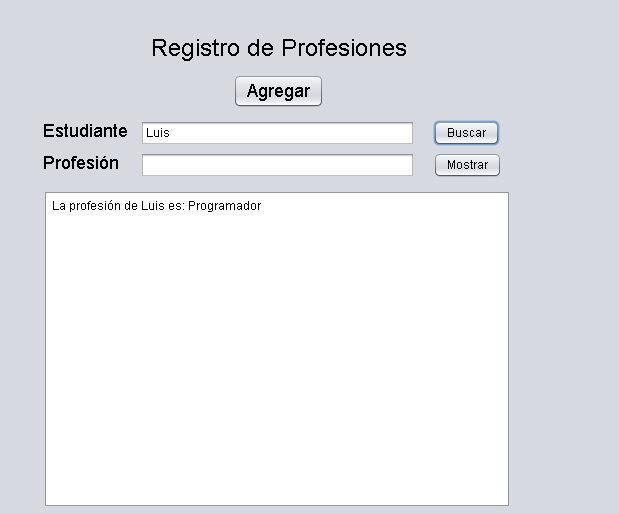
\includegraphics[width=0.8\textwidth]{assets/a12.png}
  \caption{Tercera muestra}
  \label{fig:search-data-3}
\end{figure}

\section{Documentación de la Implementación Cliente - Ciudad}

Se sigue el mismo proceso de la implementación anterior, se crea una nueva interfaz llamada Ventana 2, se agregan los botones de agregar, buscar y mostrar, y se agregan los datos solicitados.

\subsection{Generación de la interfaz}

\begin{figure}[H]
  \centering
  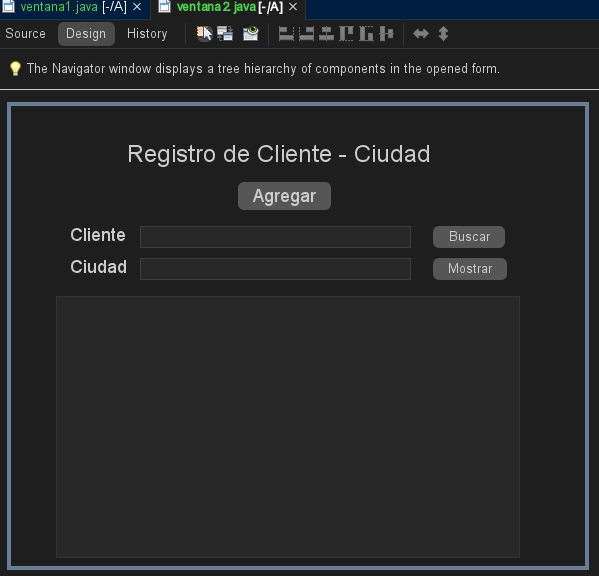
\includegraphics[width=0.5\textwidth]{assets/b1.png}
  \caption{Generación de la interfaz de cliente - ciudad}
  \label{fig:interface-generation-2}
\end{figure}

\subsection{Botón de agregar}
\begin{figure}[H]
  \centering
  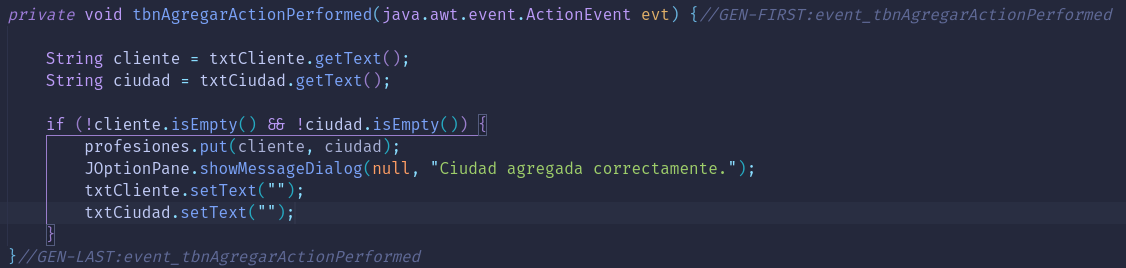
\includegraphics[width=1\textwidth]{assets/b2.png}
  \caption{Agregar datos a la tabla hash de cliente - ciudad}
  \label{fig:add-data-2}
\end{figure}
\subsection{Botón de buscar}
\begin{figure}[H]
  \centering
  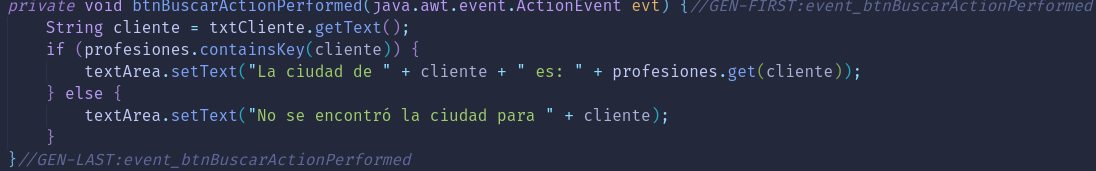
\includegraphics[width=1\textwidth]{assets/b3.png}
  \caption{Buscar datos en la tabla hash de cliente - ciudad}
  \label{fig:search-data-4}
\end{figure}
\subsection{Botón de mostrar}
\begin{figure}[H]
  \centering
  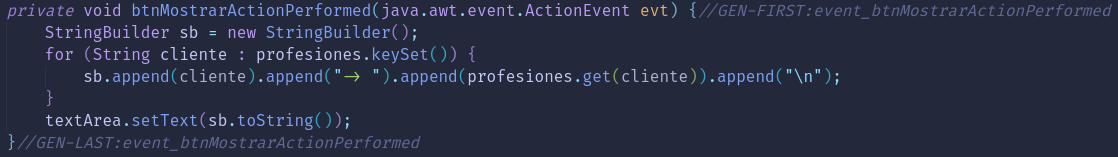
\includegraphics[width=1\textwidth]{assets/b4.png}
  \caption{Mostrar datos en la tabla hash de cliente - ciudad}
  \label{fig:show-data-2}
\end{figure}
\subsection{Agregar datos}
\begin{figure}[H]
  \centering
  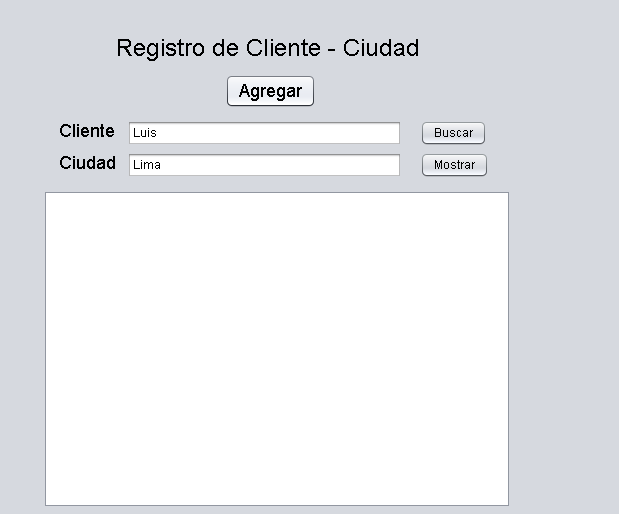
\includegraphics[width=0.6\textwidth]{assets/b5.png}
  \caption{Agregar datos a la tabla hash de cliente - ciudad}
  \label{fig:add-data-3}
\end{figure}
\begin{figure}[H]
  \centering
  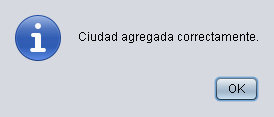
\includegraphics[width=0.3\textwidth]{assets/b6.png}
  \caption{Éxito al agregar datos a la tabla hash de cliente - ciudad}
  \label{fig:add-data-4}
\end{figure}
\subsection{Muestra de 20 Registros}
\begin{figure}[H]
  \centering
  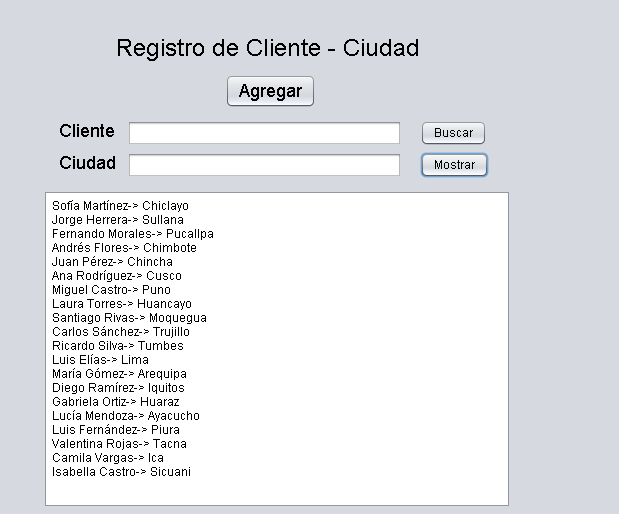
\includegraphics[width=0.7\textwidth]{assets/b7.png}
  \caption{Muestra de 20 registros en la tabla hash de cliente - ciudad}
  \label{fig:show-data-3}
\end{figure}
\subsection{Muestra de 3 búsquedas}
\begin{figure}[H]
  \centering
  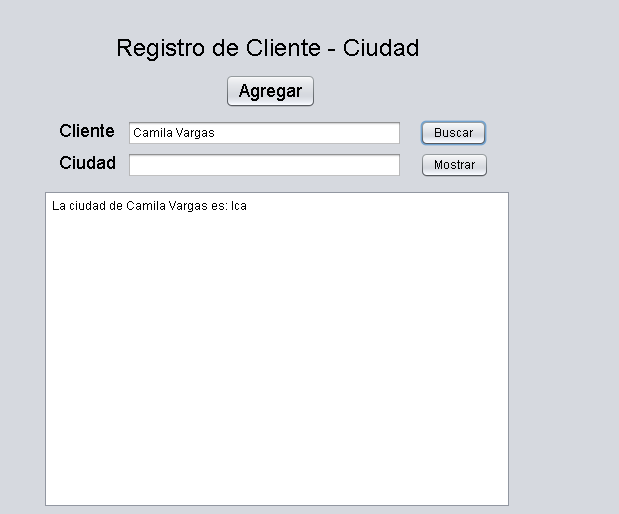
\includegraphics[width=0.7\textwidth]{assets/b8.png}
  \caption{Primera muestra de búsqueda en la tabla hash de cliente - ciudad}
  \label{fig:search-data-5}
\end{figure}
\begin{figure}[H]
  \centering
  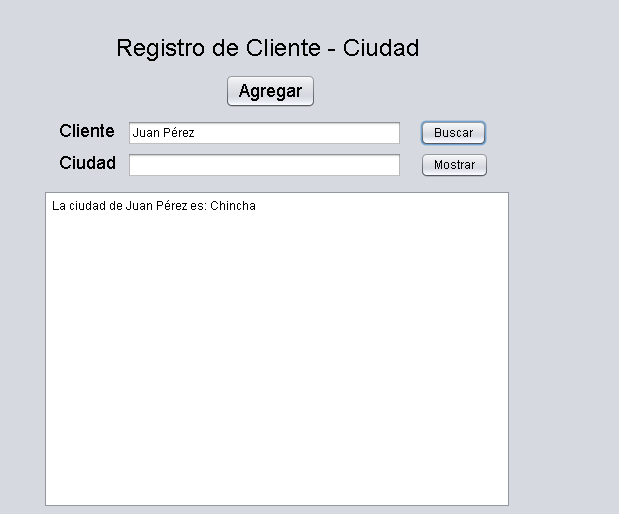
\includegraphics[width=0.8\textwidth]{assets/b9.png}
  \caption{Segunda muestra de búsqueda en la tabla hash de cliente - ciudad}
  \label{fig:search-data-6}
\end{figure}
\begin{figure}[H]
  \centering
  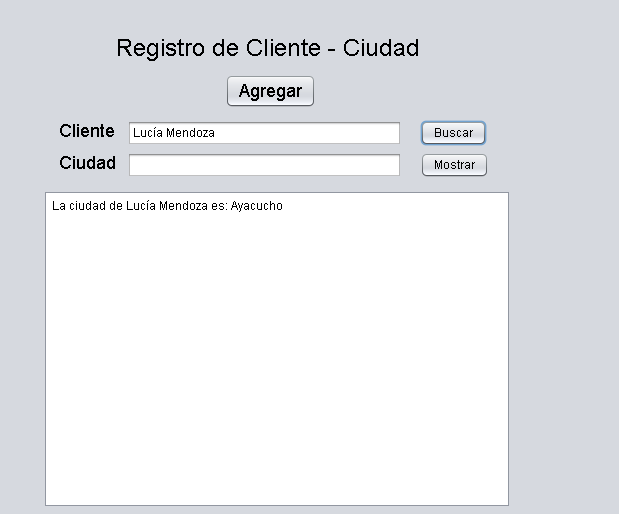
\includegraphics[width=0.8\textwidth]{assets/b10.png}
  \caption{Tercera muestra de búsqueda en la tabla hash de cliente - ciudad}
  \label{fig:search-data-7}
\end{figure}
\newpage
\section{Conclusión}
Las tablas hash son una estructura de datos eficiente para almacenar y recuperar datos gracias a la implementación de una función hash que asigna una clave que representa una dirección de memoria dado un valor como entrada.